\definecolor{bblue}{HTML}{4F81BD}
\definecolor{rred}{HTML}{C0504D}
\definecolor{ggreen}{HTML}{9BBB59}
\definecolor{ppurple}{HTML}{9F4C7C}
\newcommand*\rot{\rotatebox{90}}
\newcommand{\xmark}{\ding{55}}

This section starts with the novel framework for evaluating pointer-safety systems.
I draw up a list of criteria upon which they can be judged and comment on the patterns across the related work.

To place Bandage within the framework, I evaluated the resulting binaries from the tranformations for performance and binary size, showing them to be comparable with the current state of the art.
I then benchmarked the transformations themselves to show it runs in a reasonable time and would be capable of scaling to real life projects.

%To investigate the interactions with optimization passes, I performed further benchmarks in the presence of LLVM's O1 optimizations.
Finally, to show the security benefit that can be gained from the additional robustness to pointer-based errors that Bandage can provide, I reiterate through the examples from the Background section, commenting on Bandage's successes and short-falls.

\section{Pointer-Safety System Evaluation Framework}

The following factors are taken into account when assessing a pointer safety system:

\subsection{Spatial Safety}

\paragraph{Invalid Memory Accesses} are important to detect as they are never intentional, definitely bugs are potential security vulnerabilities.
Some systems, such as Baggy Bounds checking fail to fulfill this criterion because they only aim to prevent dangerous invalid memory accesses (such as those to a different object).

\paragraph{Incorrect Object Accesses} are when a pointer current points to an object that it was not derived from.
The Heapmon and Address Sanitizer systems fail to meet this criterion because they only track valid and invalid memory, and do not map between pointers and the memory that is valid for that pointer.
Address Sanitizer does use techniques to make the likelihood of this happening very small (by adding poisoned areas around objects).

\paragraph{Checking all variables} can be achieved through one of two methods, either by whole program analysis that lowers compatibility or by tracking calls to malloc and free in the compiled binary.
The HardBound, SoftBound and Bandage systems fail to provide this because they do not require recompilation of included libraries, and therefore do not have bounds information for pointers from them, unless the entire program is recompiled.
Baggy Bounds checking only checks the bounds of strings as an optimization strategy.

\subsection{Temporal Safety}

\paragraph{Use-After-Free Accesses} prevents dangling pointers and double frees.
I implemented a very simple case of this in the Bandage system, enough to catch simple bugs, however it is not complete, because when a copy of a pointer is freed, the original is not marked as invalid.
It is implemented in Cyclone through restrictions on the language and checks at compile time.
It is trivial to implement in systems that track valid memory areas, but not their associated pointers, such as Heapmon and Address Sanitizer.

\paragraph{Dead Stack Memory Accesses} are a similar case to that above, except the memory is released when the function returns instead of through an explicit function call.
As an aspect of temporal pointer safety, it is outside the scope of bandage.

\subsection{Binary Compatibility}

\paragraph{Program Recompilation} is required by systems that need to add hooks to the code or change its memory layout.
Most systems require program recompilation and there is a limit to the protection that can be achieved without seeing what is going on inside the program.
Body Armor for Binaries gets around this reverse engineering the program file to try to reconstruct symbol tables and such.

\paragraph{Whole Program Recompilation} requires the program and all of its included libraries to be compiled with the system.
This is linked with the \textbf{Checking all variables} criteria as a key trade-off between completeness and compatibility, especially with systems that can be run without whole program recompilation, but provide far less security when they do so.

\paragraph{Non-conforming Code Rewrite} is required by the Jones and Kelly system that overwrites the results of pointer arithmetic that exceeds the referent to the constant \verb!-2!.
This would be a valid transformation for programs that adhered strictly to the C standard, but it was found that 60\% of programs tested relied on undefined behaviour, that this broke \cite{ruwase2004practical}.

\paragraph{Code Rewrite} is the poorest level of compatibility as all programs will require some form of modification to get the system to work with them.
Cyclone requires this, due to it being a dialect of C and not a system to be run on C itself.

\begin{table}
\centering
\begin{tabular}{l|ccccccccccc}
Safety Guarantee & \rot{Bandage (FP)} & \rot{Bandage (LT)} & \rot{CCured} & \rot{SoftBound} & \rot{HardBound} & \rot{Jones \& Kelly} & \rot{Cyclone} & \rot{Heapmon} & \rot{Address San.} & \rot{Baggy Bounds} & \rot{MPX} \\
\hline
Invalid Memory Accesses        &&&&&&&&\xmark&&\xmark& \\
Incorrect Object Accesses      &&&&&&&&\xmark&\xmark&&\xmark\\
Checks All Variables            &\xmark&\xmark&&\xmark&\xmark&\xmark&&&&\xmark&\xmark\\
\hline
Use-After-Free Accesses         &*&&\xmark&\xmark&\xmark&&&&&&\xmark\\
Dead Stack Memory Accesses     &&\xmark&\xmark&\xmark&\xmark&&&\xmark&\xmark&&\xmark\\
\hline
Code Recompilation          &&\xmark&\xmark&\xmark&\xmark&\xmark&\xmark&&\xmark&\xmark&\xmark\\
Library Recompilation       &&&\xmark&&\xmark&&\xmark&&&&\xmark\\
Non-conforming Code Rewrite   &&&&&&\xmark&&&&&\\
Code Rewrite                &&&&&&&\xmark&&&&\\
\end{tabular}
\caption{Safety guarantees for evaluated pointer safety systems. A cross indicates the guarantee is \textbf{not} provided.}
\label{fig:TickTable}
\end{table}

The evaluated systems are marked according to the previous criteria in Table \ref{fig:TickTable}.

\subsection{Runtime Overhead}

\paragraph{Runtime Overhead} is the current leading method for comparing pointer-safety systems, probably due to its quantitative and easy to measure nature.
It is important, and therefore I've included it, however as can be seen in Table \ref{fig:Others}, most systems (those that do not require hardware assistance) perform comparably.

\subsection{Extra Requirements}

\paragraph{Hardware Support} may be required by the system.
This likely signifies that the system will not be very compatible - a full program analysis is likely to be required for full coverage.
Additionally the cost of the new hardware must be factored in, making it unrealistic for projects such as those designed for widespread use on personal computers.

\paragraph{Additional Threads} could be an issue if the target program is desired to be run on less powerful systems.
An additional thread running may require more resources that aren't made explicit in the benchmarks.

I have summarized the extra requirements and runtime overheads imposed by each tool in Table \ref{fig:Others}.

Together these tables provide a full picture of the relative strengths and weaknesses of these tools, allowing programmers to make an informed decision over which is the best for the task at hand.
A programmer with a non-real time legacy system could start by choosing Heapmon and accept the runtime overhead as an acceptable price for the lack of compilation time overhead.
Alternatively a programmer looking to write a secure system from scratch would be well advised to use Cyclone (provided the garbage collector isn't an issue).

\begin{table}
\centering
\begin{tabular}{l|r|r}
System & Runtime Overhead & Extra Requirements \\
\hline
Bandage (FP)            &Up to 100\%&\\
Bandage (LT)            &Up to 300\%&\\

CCured              &Up to 250\%&\\
SoftBound           &Up to 350\%&\\
HardBound           &Up to 25\%&Hardware\\
Jones \& Kelly      &Not Reported&\\
Cyclone             &Up to 250\%&Garbage Collector\\
HeapMon             &Up to 450\%&Extra Thread\\
Address Sanitizer   &Typically 200\%&\\
Baggy Bounds        &Up to 230\%&\\
MPX                 &None Available&Hardware\\
\end{tabular}
\caption{Runtime and extra requirements of evaluated pointer safety systems.}
\label{fig:Others}
\end{table}

\section{Transformed Code Performance}

The following benchmarks were carried out on an 8 core, 64bit, 3.6GHz Intel Xeon CPU, running FreeBSD 10.0.
In addition to the benchmarks, Bandage was developed using a suite of 54 tests, including a few complex tests along with unit tests for:

\begin{itemize}
\item Array operations
\item Pointer operations
\item Function boundary transitions
\item Compatibility with C libraries
\item Correct identification of pointers for the analysis pass.
\end{itemize}

\subsection{Microbenchmarks}

A selection of tailored micro benchmarks were created to investigate the effects of the transformation on individual parts of code.

\subsubsection{Safe Pointer Dereference}

\begin{minted}[fontsize=\footnotesize,frame=single]{c}
// Setup
int x;
int y=malloc(sizeof(int));
// Benchmarked Code
x=*y;
\end{minted}

As \verb!y! is recognised as a safe pointer, no bounds checking will be carried out, however a null check is performed.
This null check incurs an overhead of $4.6\% \pm 0.3\%$.

If there null check were omitted, the only overhead of the fat pointer approach would be the load required to retrieve the fat pointer value.
This benchmark was run without the null check, and the load was found to incur an overhead of $0.92\% \pm 0.11\%$.

\subsubsection{Unsafe Pointer Dereference}

\begin{minted}[fontsize=\footnotesize,frame=single]{c}
// Setup
int x;
int *y=malloc(3*sizeof(int));
x=y[1];
// Benchmark Code
x=*y;
\end{minted}

By using array addressing on the pointer, the pointer analysis detects \verb!y! as a pointer that has arithmetic done on it, and is therefore not \textit{SAFE}.
Therefore the pointer dereference will contain the full bounds check, that was found to incur an overhead of $52\% \pm 2.4\%$.

The bounds check function used was complex, first it checked if the value was null, then if the base was null (signifying a pointer of type \textit{NoBounds!}, and finally if the value were within the base and bound.

\subsubsection{Pointer Allocation}

\begin{minted}[fontsize=\footnotesize,frame=single]{c}
// Setup
void Fun1(){}
void Fun2(){int *a,*b,...,*j;}
\end{minted}

Many calls were made to \verb!Fun1! and to \verb!Fun2! and the difference in execution time was measured.
This benchmark needed to be done this way because memory used by an allocation is not free until the scope it is allocated in is left, therefore if the allocation were performed in a loop, the stack would run out of space.
This was found to produce no measurable difference.

\subsubsection{Pointer Assignment}

\begin{minted}[fontsize=\footnotesize,frame=single]{c}
// Setup
int *a,*b;
// Benchmark Code
a=b;
\end{minted}

There is no bounds checking on this code as no pointers are dereferenced, its purpose is to observe the overhead of copying three pointers instead of one.
This was found to produce no measurable difference.

\subsubsection{Following a Linked List}

This benchmark was created to highlight the difference between the fat pointer and the lookup table approach, because with my lookup table implementation no lookup occurs for local variables.
A linked chain is created and then followed.
These tests were repeated with a linked lists of different lengths to investigate how each approach scales with the number of pointers that it needs to keep track of.

Figure \ref{fig:LinkedListScaling} shows the results (the errors were negligible).
The first and most obvious result is that, now that the pointers are stored on the heap and therefore table lookups are required for pointer bounds the table lookup approaches are slower than the fat pointer approach.

\begin{figure}
\centering
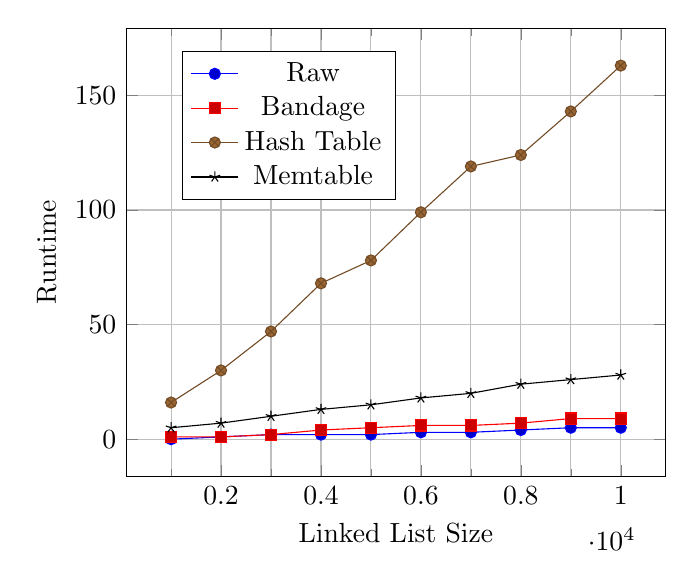
\begin{tikzpicture}
  \begin{axis}[ 
      xlabel=Linked List Size,
      ylabel=Runtime,
      minor x tick num=1,
      grid=both,
	  legend style={at={(0.5,0.95)}}
    ] 
    \addplot coordinates{
		(	1000	,	0	)
		(	2000	,	1	)
		(	3000	,	2	)
		(	4000	,	2	)
		(	5000	,	2	)
		(	6000	,	3	)
		(	7000	,	3	)
		(	8000	,	4	)
		(	9000	,	5	)
		(	10000	,	5	)
    }; 
	\addlegendentry{Raw}
    \addplot coordinates{
		(	1000	,	1	)
		(	2000	,	1	)
		(	3000	,	2	)
		(	4000	,	4	)
		(	5000	,	5	)
		(	6000	,	6	)
		(	7000	,	6	)
		(	8000	,	7	)
		(	9000	,	9	)
		(	10000	,	9	)
    }; 
	\addlegendentry{Bandage}
    \addplot coordinates{
		(	1000	,	16	)
		(	2000	,	30	)
		(	3000	,	47	)
		(	4000	,	68	)
		(	5000	,	78	)
		(	6000	,	99	)
		(	7000	,	119	)
		(	8000	,	124	)
		(	9000	,	143	)
		(	10000	,	163	)
	}; 
	\addlegendentry{Hash Table}
    \addplot coordinates{
		(	1000	,	5	)
		(	2000	,	7	)
		(	3000	,	10	)
		(	4000	,	13	)
		(	5000	,	15	)
		(	6000	,	18	)
		(	7000	,	20	)
		(	8000	,	24	)
		(	9000	,	26	)
		(	10000	,	28	)
	}; 
	\addlegendentry{Memtable}
  \end{axis}
\end{tikzpicture}
\caption{Increase in runtime following a Linked List as size increases}
\label{fig:LinkedListScaling}
\end{figure}


The hash table performs the worst with a \verb!32x! runtime increase at the largest list size.
This is not surprising considering that each lookup requires a look through each bucket for the matching element.
The interesting result is that the runtime seems to increase linearly with the list size, implying a close to $O(1)$ overhead for hashtable lookup.

With the longest linked list length, the MemTable takes five times as long as with no bounds checking and three times longer than bandage.
The MemTable lookup consists of pointer arithmetic and an access to the \verb!mmap!ed area, whereas a fat pointer lookup consists of and a load from a structure.
A potential reason the MemTable approach takes longer than fat pointers is that an iteration for the fat pointer contains a load that fetches both the next pointer value and its bound at the same time, and they are store contiguously in memory.
An iteration with MemTables consists of a lookup to find the next pointer, and then a lookup in the table to find the bounds for that pointer, requiring two lookups to two areas of memory that are likely very far apart.

As the linked list was allocated in order, each element is likely arranged sequentially in memory.
Therefore, because the MemTable uses the pointer's address in memory as the index to that pointer's information, the bounds information associated with each linked list item will also be arranged sequentially in memory, and quite close together, giving very good spatial locality for the caches to take advantage of.

Finally, because the table lookup functions are compiled separately and linked with the code, function inlining is prevented.
This would result in more branching.

A summary of the microbenchmarks can be found in Table \ref{fig:Micros}.

\begin{table}
\centering
\begin{tabular}{|lrr|}
\hline  Benchmark & Fat Pointer Overhead & Lookup Table Overhead\\
\hline
Safe Dereference    & \text{$4.6\% \pm 0.3\%$}     & Same as Fat Pointer \\
Unsafe Deference    & \text{$52\% \pm 2.4\%$}     & Same as Fat Pointer \\
Allocation          & Negligible     & Same as Fat Pointer \\
Assignment          & Negligible     & Same as Fat Pointer \\
Linked List         & \text{$110\% \pm 7\%$}     & \text{$410\% \pm  19\%$} \\
\hline
\end{tabular}
\caption{Fat pointer and lookup table overheads compared to uninstrumented runtime for the microbenchmarks.}
\label{tab:Micros}
\end{table}

\subsection{Olden Benchmarks}

The Olden suite of benchmarks are designed to benchmark pointer-heavy data structures \cite{olden}.
Due to the complex nature of the transformation (especially the fat pointer transformation), some of the Olden benchmarks are not transformed correctly, and fail to run (\verb!em3d!, \verb!health!, \verb!bh!, \verb!mst!).
This is due to issues with the implementation of Bandage, and not due to limits in the system.

Most of the benchmarks center around constructing binary trees (each node contains pointers to two other nodes, and a value), for example the treeadd benchmark constructs a tree and performs a depth-first search to accumulate all the values and the bisort benchmark performs a binary merge at each node to sort the tree.
The results of the benchmarks are shown in Table \ref{tab:OldenRuntime} and Figure \ref{fig:OldenRuntime}.
These results show performances comparable to those of the state of the art research papers, with the fat pointer implementation not exceeding 200\% of the original runtime in any benchmark.
The runtimes for the lookup table approach were measured with the memtable implementation, though this still produced a greater overhead (if in part due to the inability to inline the lookup functions as they were included from a different library).

\begin{table}
\centering
\begin{tabular}{|lrr|}
\hline  Benchmark & Fat Pointer Overhead & Lookup Table Overhead\\
\hline
Bisort      & \text{$71\% \pm 1\%$}     & \text{$164\% \pm  1\%$} \\
Perimeter   & \text{$35\% \pm 7\%$}     & \text{$294\% \pm 11\%$} \\
Power       & \text{$46\% \pm 1\%$}     & \text{$101\% \pm  1\%$} \\
Treeadd     & \text{$49\% \pm 4\%$}     & \text{$253\% \pm  6\%$} \\
Tsp         & \text{$95\% \pm 2\%$}     & \text{$211\% \pm  3\%$} \\
\hline
\end{tabular}
\caption{Fat pointer and lookup table overheads compared to uninstrumented runtime for the Olden benchmarks.}
\label{tab:OldenRuntime}
\end{table}
\begin{figure}
\centering
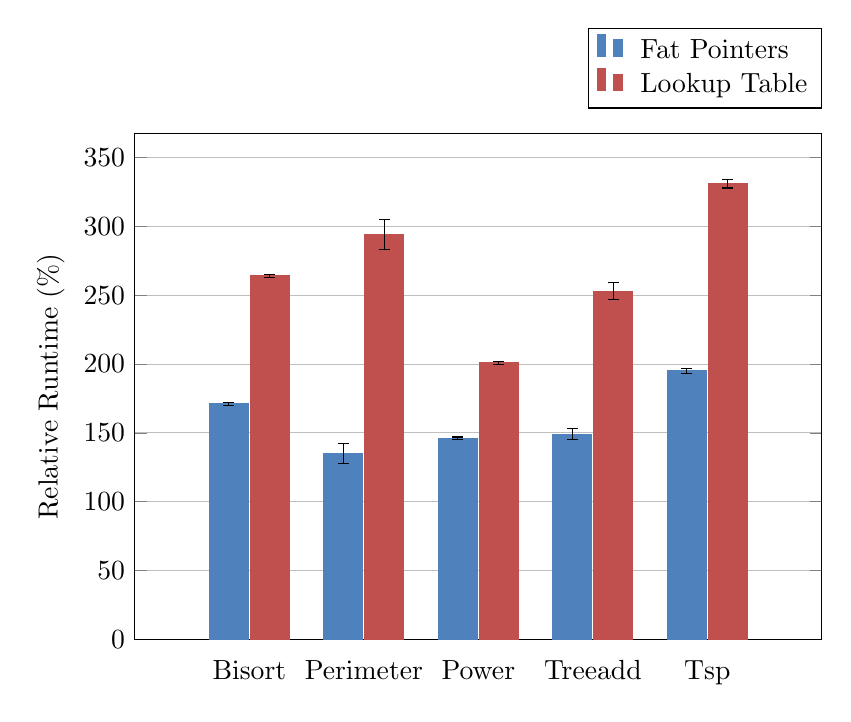
\begin{tikzpicture}
    \begin{axis}[
        width  = 0.85*\textwidth,
        height = 8cm,
        major x tick style = transparent,
        ybar=2*\pgflinewidth,
        bar width=14pt,
        ymajorgrids = true,
        ylabel = {Relative Runtime (\%)},
        symbolic x coords={Bisort,Perimeter,Power,Treeadd,Tsp},
        xtick = data,
        scaled y ticks = false,
        enlarge x limits=0.25,
        ymin=0,
        legend cell align=left,
        error bars/error bar style={black},
        legend style={
                at={(1,1.05)},
                anchor=south east,
                column sep=1ex
        }
    ]
        \addplot[
            fill=bblue,
            draw=bblue,
            error bars/.cd,
            y dir=both,
            y explicit]
        table [y error=error]{
            x           y       error
            Bisort      171     1
            Perimeter   135     7
            Power       146     1
            Treeadd     149     4
            Tsp         195     2
        };

        \addplot[
            fill=rred,
            draw=rred,
            error bars/.cd,
            y dir=both,
            y explicit]
        table [y error=error]{
            x           y       error
            Bisort      264     1
            Perimeter   294     11
            Power       201     1
            Treeadd     253     6
            Tsp         331     3
        };
        \legend{Fat Pointers, Lookup Table}
    \end{axis}
\end{tikzpicture}
\caption{Graphical representation of relative runtime for Olden benchmarks.}
\label{fig:OldenRuntime}
\end{figure}


%\subsubsection{Treeadd}
%
%The treeadd benchmark constructs a binary tree where each node contains a value in addition to two children (all values are set to 1).
%A depth-first search is then performed, accumulating the value at each node.
%
%The implementation of CCured-like analysis counts all member pointers as a non-SAFE type (because the actions on the pointer and therefore the CCured type will be different for each instance), meaning that the tree traversal doesn't benefit from CCured-analysis.
%
%Under Bandage, the tree construction stage, dominated by memory allocations took a \verb!42%! performance hit and the tree traversal stage took a \verb!77%! performance hit.
%
%% 744809 223446 968255
%% 1060893 395186 1456079
%% Unoptimized bounds checking
%
%\subsubsection{Bisort}
%
%The bisort benchmark constructs a binary tree with each node containing a random value.
%The tree is then sorted by performing a binary merge at each node, working up to the root node.
%
%Under Bandage, tree construction displayed little overhead with a \verb!3%! slowdown, though the sorting caused a larger overhead of \verb!165%!, resulting in an overall runtime increase of \verb!83%!.
%
%\subsubsection{Mst}
%\subsubsection{Perimeter}
%\verb!-8%!
%\verb!23%!
%\verb!-3%!
%\subsubsection{Power}
%\subsubsection{Tsp}
%
%The tsp benchmark constructs a 2d tree of nodes and proceeds to solve the travelling salesman problem.
%For nodes close together, it uses the closest pointer heuristic.
%
%Under Bandage, tree construction introduced no overhead but application of the travelling salesman problem increased runtime by \verb!103%!.

\subsubsection{Failing Benchmarks}

Due to the complex nature of the transformation (especially the fat pointer transformation), some of the Olden benchmarks are not transformed correctly.
There is overlap with the benchmarks evaluated for the CHERI paper, with \verb!bisort!, \verb!perimeter! and \verb!treeadd! working for both CHERI and Bandage, \verb!mst! working for CHERI but not Bandage and \verb!power! and \verb!tsp! working for Bandage and not CHERI.

%\subsubsection{Type Coercion}

%One of reasons that the benchmarks fail to run is Type Coercion.
%In some circumstances, the LLVM IR produced by clang coerces the types of parameters to functions.
%For example, the \verb!em3d! benchmark contains the following function:
%
%\begin{minted}[fontsize=\footnotesize,frame=single]{c}
%typedef struct node_t{
%    double value;
%} node_t;
%
%typedef struct graph_t{
%    node_t *e;
%    node_t *h;
%} graph_t;
%
%void print_graph(graph_t graph){...}
%\end{minted}
%
%Instead of the struct being passed to the function as a whole struct, it is split into its two members and the function in IR actually takes two \verb!node_t *!s as its parameters, which are then put into a anonymous type of \verb!{node_t *, node_t *}! which is finally bitcast into a \verb!graph_t!.

\section{Compile-time Performance}

I timed the compilation for the Olden benchmarks for both transformations.
The results, shown in Figure \ref{fig:CompTime} show that the fat pointer transformation is usually quicker than the lookup table transformation, but both transformations are always in the same order of magnitude of raw compilation and frequently take less than twice its length.
\begin{figure}
\centering
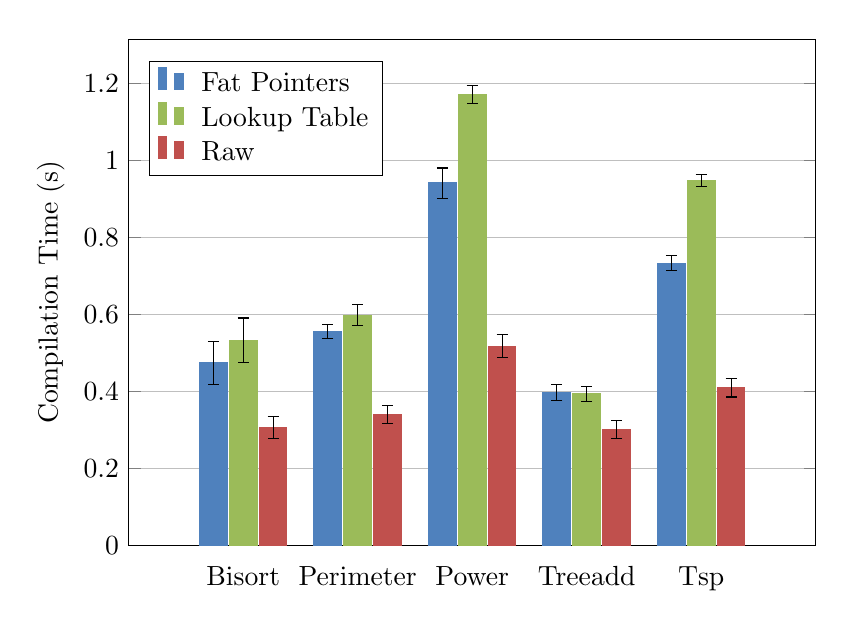
\begin{tikzpicture}
    \begin{axis}[
        width  = 0.85*\textwidth,
        height = 8cm,
        major x tick style = transparent,
        ybar=2*\pgflinewidth,
        bar width=10pt,
        ymajorgrids = true,
        ylabel = {Compilation Time (s)},
        symbolic x coords={Bisort,Perimeter,Power,Treeadd,Tsp},
        xtick = data,
        scaled y ticks = false,
        enlarge x limits=0.25,
        ymin=0,
        legend cell align=left,
        error bars/error bar style={black},
        legend style={
                at={(0.37, 0.73)},
                anchor=south east,
                column sep=1ex
        }
    ]
        \addplot[
            fill=bblue,
            draw=bblue,
            error bars/.cd,
            y dir=both,
            y explicit]
        table [y error=error]{
            x           y       error
            Bisort      0.4733     0.0562
            Perimeter   0.5551     0.0182
            Power       0.9405     0.0390
            Treeadd     0.3964     0.0213
            Tsp         0.7323     0.0192
        };

        \addplot[
            fill=ggreen,
            draw=ggreen,
            error bars/.cd,
            y dir=both,
            y explicit]
        table [y error=error]{
            x           y       error
            Bisort      0.5324     0.0576
            Perimeter   0.5975     0.0279
            Power       1.17	   0.0233
            Treeadd     0.393      0.0201
            Tsp         0.9466     0.0155
        };

        \addplot[
            fill=rred,
            draw=rred,
            error bars/.cd,
            y dir=both,
            y explicit]
        table [y error=error]{
            x           y       error
            Bisort      0.3049     0.0284
            Perimeter   0.3395     0.0231
            Power       0.5169     0.0303
            Treeadd     0.2996     0.0232
            Tsp         0.4091     0.0244
        };

        \legend{Fat Pointers, Lookup Table, Raw}
    \end{axis}
\end{tikzpicture}
\caption{Compilation time for Olden benchmarks.}
\label{fig:CompTime}
\end{figure}

I measured the resulting binaries, finding that the transformation produced a greater increase in binary size than in compilation time (Figure \ref{fig:BinSize}).
The binary sizes for both of the transformations were both quite similar, indicating that the primary increase in binary size was due to the common operations shared between the transformations, such as calculating bounds and calling the bounds checking functions.

\begin{figure}
\centering
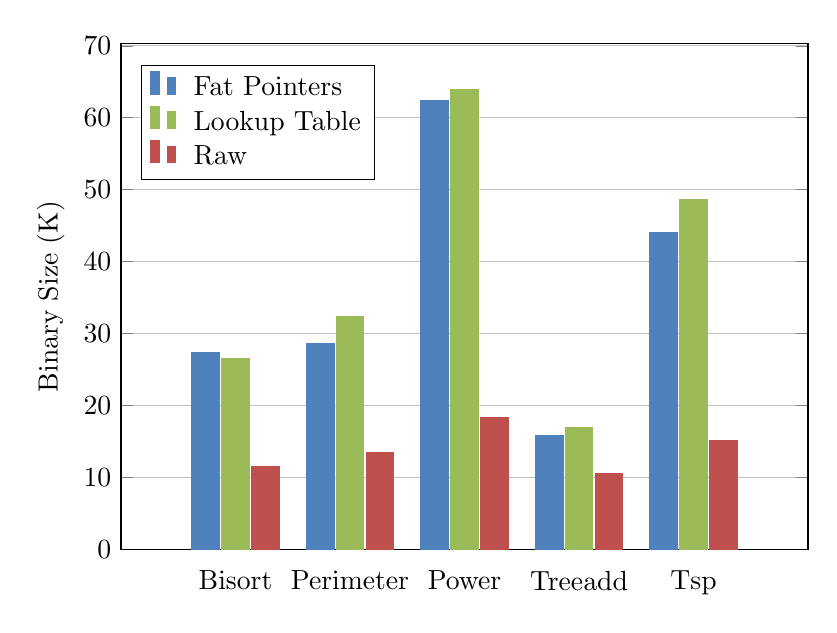
\begin{tikzpicture}
    \begin{axis}[
        width  = 0.85*\textwidth,
        height = 8cm,
        major x tick style = transparent,
        ybar=2*\pgflinewidth,
        bar width=10pt,
        ymajorgrids = true,
        ylabel = {Binary Size (K)},
        symbolic x coords={Bisort,Perimeter,Power,Treeadd,Tsp},
        xtick = data,
        scaled y ticks = false,
        enlarge x limits=0.25,
        ymin=0,
        legend cell align=left,
        legend style={
                at={(0.37, 0.73)},
                anchor=south east,
                column sep=1ex
        }
    ]
        \addplot[style={bblue,fill=bblue,mark=none}]
            coordinates {(Bisort,   27.287) (Perimeter,   28.631) (Power,   62.375) (Treeadd,   15.850) (Tsp,   44.090)};

        \addplot[style={ggreen,fill=ggreen,mark=none}]
            coordinates {(Bisort,   26.546  ) (Perimeter,   32.325  ) (Power,   63.873) (Treeadd,   16.930) (Tsp,   48.570  )};

        \addplot[style={rred,fill=rred,mark=none}]
            coordinates {(Bisort,   11.535  ) (Perimeter,   13.445  ) (Power,   18.293  ) (Treeadd,   10.590  ) (Tsp,   15.104  )};
        \legend{Fat Pointers, Lookup Table, Raw}
    \end{axis}
\end{tikzpicture}
\caption{Binary size of Olden benchmarks.}
\label{fig:BinSize}
\end{figure}


%\section{Interactions with Optimizations passes}
%
%Since many optimizations rely on each other and inter-react, instead of individually enabling optimizations, I individually disabled them.
%Table \ref{tab:Opts} shows the performance difference when the tsp benchmark (picked as it produced the highest runtime increase itself) was run with the stated optimizations disabled.
%All of the optimizations used in O1 optimization were run 10 times and only those that produced a difference of greater than \verb!5%! are shown in the table.
%
%Since the stated optimizations were omitted, a beneficial optimization would give a negative value in the table - showing that its omission caused the resulting binary to take longer to execute.
%The table shows that most optimizations give a negative result when applied to the fat pointer code.
%
%%\begin{table}
%%\centering
%%\begin{tabular}{|lrr|}
%%\hline Omitted Optimization & Raw Speedup & Fat Pointer Speedup \\
%%\hline
%%early-cse   &   \verb!-3.30%! &   \verb!22.29%!   \\
%%instcombine &   \verb!5.48%!  &   \verb!7.56%!    \\
%%loop-rotate &   \verb!-1.28%! &   \verb!9.94%!    \\
%%simplifycfg &   \verb!-2.47%! &   \verb!-5.75%!   \\
%%sroa        &   \verb!0.23%!  &   \verb!7.45%!    \\
%%\hline
%%\end{tabular}
%%\caption{Performance Differences on the Tsp benchmark with selection optimizations disabled}
%%\label{tab:Opts}
%%\end{table}
%
%\begin{table}
%\centering
%\begin{tabular}{|lrrrr|}
%\hline &   sroa    &   loop-rotate &   loop-unroll &   instcombine \\
%\hline
%bisort&\verb!19.06%!&\verb!-0.90%!&\verb!0.34%!&\verb!5.13%!\\
%power&\verb!3.01%!&\verb!18.54%!&\verb!7.71%!&\verb!-0.33%!\\
%perimeter&\verb!17.46%!&\verb!1.62%!&\verb!-2.51%!&\verb!1.26%!\\
%treeadd&\verb!12.84%!&\verb!-0.30%!&\verb!0.93%!&\verb!-1.37%!\\
%tsp&\verb!-7.32%!&\verb!-9.56%!&\verb!-0.14%!&\verb!-7.97%!\\
%\hline
%\end{tabular}
%\caption{Performance Differences on the Olden benchmarks with selection optimizations disabled}
%\label{tab:Opts}
%\end{table}
%
%\subsection{Scalar Replacement of Aggregates}
%
%Scalar replacement of aggregates is a function based optimization that aims to separate aggregates, such as structs and arrays into simple components which can then be assigned to temporary values.
%These temporary values can then be the target of further optimizations such as register allocation and copy or constant propegation \cite[Chapter~12]{steven1997advanced}.
%
%One of the actions of this pass is to replace some member accesses with \verb!extractvalue! and \verb!insertvalue! instructions \cite{llvmSROA}, for example in the following code:
%
%\begin{minted}[fontsize=\footnotesize,frame=single]{llvm}
%%1 = alloca %FatPointer
%%2 = getelementptr %FatPointer* %Ptr, i32 0, i32 1
%store i32* null, i32** %2
%%3 = getelementptr %FatPointer* %Ptr, i32 0, i32 2
%store i32* null, i32** %3
%\end{minted}
%
%\begin{minted}[fontsize=\footnotesize,frame=single]{llvm}
%%1 = alloca %FatPointer
%%2 = insertvalue %FatPointer %Ptr, i32* null, 1
%%3 = insertvalue %FatPointer %Ptr, i32* null, 2
%\end{minted}
%
%The \verb!insertvalue! instruction returns a pointer to the updated struct, which is then used in further code.
%This simplifies the dependency graph, making each subsequent field assignment dependant on the last (so \verb!%3! depends on \verb!%2! which depends on \verb!%1!) instead of all dependant on the \verb!alloca! at the top.
%
%Usually with this pass, the \verb!alloca! instruction at the top is removed entirely, because where originally there was an \verb!alloca!, then a call to \verb!malloc! then an assignment to the allocated variable, there is now only a call.
%Unfortunately, both of the Bandage transformation passes rely on the \verb!alloca! instructions at the start of each function to gather the variables, so this pass cannot be performed before the transformation.
%The fat pointer pass transforms variables into their fat pointer versions at this point, and the lookup table pass registers them as local variables and generates their local bounds.
%
%Without this optimization, fat pointers as aggregate objects will be ineligable for many future transformations, which would be very detrimental considering the prevalence of pointers in many C programs.
%With it, for the purposes of future, function based optimzations a fat pointer can be seen as three separate scalar variables.
%
%\subsection{Instruction Combination}
%
%Instruction combination is a simple worklist driven algorithm that looks for opportunities to simplify the code, for example by replacing multiplications by powers of two with shift operations.
%Like with SROA, the primary benefit of this pass is that it allows future optimizations to be more effective.
%
%\subsection{Overhead due to Cache and Register Churn}
%
%Bandage was modified to not insert bounds or null checks on pointer dereference, and the benchmarks were run again.
%This provided a measurement of the overhead introduced by using fat pointers (and therefore dealing with the extra loads, pointer wrapping and stripping and cache overhead) and by propegating the bounds information.
%The overheads introduced here allow evaluation of the bounds checking strategy separate from those overheads and also provides a theoretical lower bound on what an optimization to the checking strategy can achieve.
%
%\begin{table}
%\centering
%\begin{tabular}{|l|r|r|}
%\hline \textbf{Olden Benchmark} & \textbf{O0 Overhead} & \textbf{O3 Overhead}\\
%\hline Bisort       &   7.50\%   &   3.44\% \\
%\hline Perimeter    & -18.62\%   & -43.49\% \\
%\hline Power        &  19.32\%   &  12.12\% \\
%\hline Treeadd      &  28.75\%   &  17.11\% \\
%\hline Tsp          &   7.29\%   &  28.57\% \\
%\hline
%\end{tabular}
%\caption{Runtime overhead on olden benchmarks when no bounds or null checks are inserted}
%\label{tab:NoChecks}
%\end{table}
%
%The runtime overheads are shown in Table \ref{tab:NoChecks}, for comparison when the code was run without optimization and when the code was run with O3.
%It is gratifying to see that in most of the cases, O3 optimization reduces the gap between uninstrumented and instrumented code.
%
%\subsubsection{Tsp interfering with Optimization}
%
%Looking at the runtime breakdown of the Tsp benchmark gives us the timings in Table \ref{tab:TspNoChecks}.
%It can be seen that large discrepancy in optimization speedups arises during the set of O1 optimizations.
%
%\begin{table}
%\centering
%\begin{tabular}{|l|r|r|}
%\hline  \textbf{Optimization Level}  &   \textbf{Raw} &   \textbf{Bandage} \\
%\hline  O1  &   20.51\%  &   -2.33\%  \\
%\hline  O2  &   26.92\%  &   13.95\%  \\
%\hline  O3  &   26.92\%  &   13.95\%  \\
%\hline
%\end{tabular}
%\caption{Speedup relative to O0 optimization for raw and bandage transformed Tsp benchmark.}
%\label{tab:TspNoChecks}
%\end{table}
%
%In order to investigate this further, O1 optimization was repeated multiple times on the uninstrumented code, each time with a specific optimization disabled, to determine which was responsible for the \verb!20%! speedup.
%Each of the resulting binaries displayed speedups of \verb!17%! or more, suggesting that no single optimization was responsible for the speedup.
%It was found however, when the \verb!instcombine! optimization was omitted, the speedup for the unoptimized binary was \verb!25%!, indicating that it actually slows the resulting program.
%
%The same process was repeated on the instrumented IR.
%It was found that with each optimization pass specified manually, a speedup of \verb!25\%! is achieved - similar to that of the raw binary, but when specified through the O1 flag, the speedup is negligable.
%
%However, this process also identified the O1 optimizations that were the most responsible for was responsible for the speedup.
%Without the \verb!instcombine! or the \verb!sroa! optimizations, the speedup dropped to \verb!1%!.
%Additionally, the absence of the \verb!early-cse! optimization caused the speedup to drop to \verb!17%!.



\section{Conclusion}

The Bandage system that I developed provides multiple backends for pointer bounds checking and allows the user to choose how much of their program they want to recompile.
It creates four new points in the design space of pointer-safety systems, shown again in Figure \ref{fig:Spectrum2} the two Bandage points on the left signify Bandage being used for a whole program transformation whereas the two on the right mark its use on just the program code (and not the libraries).
The lookup table transformation provides slightly more complete safety than the fat pointer transformation, because there are C operations that can strip the bounds information from a fat pointer (for example converting a pointer to an integer and back).
Additionally Bandage can be used as a full program analysis, that would provide bounds for pointers received from libraries.

\begin{figure}
\centering
\begin{tikzpicture}
\makeatletter
\tikzset{
    nomorepostaction/.code=\makeatletter\let\tikz@postactions\pgfutil@empty, % From http://tex.stackexchange.com/questions/3184/applying-a-postaction-to-every-path-in-tikz/5354#5354
    my axis/.style={
        postaction={
            decoration={
                markings,
                mark=at position 1 with {
                    \arrow[ultra thick]{latex}
                }
            },
            decorate,
            nomorepostaction
        },
        thin,
        -, % switch off other arrow tips
        every path/.append style=my axis % this is necessary so it works both with "axis lines=left" and "axis lines=middle"
    }
}
\makeatother

\begin{axis}[
    width=\textwidth,
    yticklabels={,,},
    xticklabels={,,},
    ticks=none,
    axis lines = left,
    axis line style=my axis,
    xmin=0,
    xmax=1,
    ymin=0,
    ymax=1,
    xlabel={Compatibility},
    ylabel={Completeness},
    ]
\addplot[
    only marks,
    mark=*,
    mark options={fill=white},
    visualization depends on=\thisrow{alignment} \as \alignment,
    nodes near coords, % Place nodes near each coordinate
    point meta=explicit symbolic, % The meta data used in the nodes is not explicitly provided and not numeric
    every node near coord/.style={anchor=\alignment}, % Align each coordinate at the anchor 40 degrees clockwise from the right edge
    ] table [% Provide data as a table
     meta index=2 % the meta data is found in the third column
     ] {
        x       y       label       alignment
        1       0.1       C           -40
        0.2     0.8     Cyclone     -40
        0.7     0.65     {Bandage (FP)}    180
        0.7     0.7     {Bandage (LT)}     180
        0.4     0.75    {Bandage (LT)}     180
        0.4     0.7     {Bandage (FP)}      180
        0.4     0.8     CCured      0
        0.7     0.6     SoftBound   -180
        0.4     0.6     HardBound   0
        0.4     0.8     CHERI       180
        0.6     0.6     J\&K        -40
        0.9     0.4     Heapmon     90
	0.9	0.3	{Body Armour} 90
        0.7     0.55    AddrSan     180
        0.7     0.5     Baggy       90
	0.7	0.4	{Practical Dynamic} 0
        0.4     0.5     MPX         0
    };
\end{axis}
\end{tikzpicture}
\caption{The completeness vs compatibility tradeoff in pointer-safety systems, including Bandage.}
\label{fig:Spectrum2}
\end{figure}



The robustness provided by the Bandage system brings with it security benefits, for example it is capable of stopping the buffer-overflow attack detailed in the Background section.

I used the Olden benchmarks to evaluate the performance overhead incurred by the Bandage transformations.
This resulted in overheads comparable to current techniques.
However, the Bandage transformation is highly modular, allowing it to be used in future research in the area, with more efficient transformations or more accurate analyses, potentially leading to it being used with lower overhead in the future.

Investigation into further optimizations revealed that the scalar replacement of aggregates pass was highly useful after the fat pointer optimization, as essentially made the value of the fat pointer available to all the optimizations that a raw pointer could take advantage of.
